\chapter{Implementierung}\label{ch:implementierung}

Die Implementierung des Systems orientiert sich sehr stark an den in Kapitel \vref{ch:konzeption} dargestellten Komponenten.
Den Anforderungen entsprechend wurde das System in objektorientiertem C++ implementiert.
Aufgrund der absehbar großen Datenmengen, die bei längeren Aufnahmezeiten entstehen, wurde als Datenbank eine SQLite3 Datenbank\betterfootcite{sqlite} gewählt, da sie einen geringen Einrichtungsaufwand verlangt, jedoch gleichzeitig ein sicheres Speichern und ein hohe Lesegeschwindigkeit bietet.
Um den Code les- und wartbarer zu gestalten wurden Funktionen des neuesten C++11 Sprachstandards\betterfootcite{stroustrup2005design} benutzt.

\section{Klassen}

\subsection{Recorder}

Der Aufnahmevorgang greift zurück auf eine trivialen Klasse \textbf{Recorder} zusammen mit den in Abbildung \vref{fig:training} dargestellten Containerklassen \textbf{Object} und \textbf{ObjectSet}.
Der Konstruktor der \textbf{Recorder}-Klasse erlaubt als Parameter lediglich die Angabe einer Zieldatei für die Datenbank.
Des Weiteren besitzt sie nur eine Methode \textbf{insert}, der ein \textbf{ObjectSet} und ein \textbf{String} mit dem Szenennamen übergeben werden, um dann in der Datenbank abgespeichert zu werden.

\subsubsection{Datenbankschema}

Das Datenbankschema für die Aufnahme ist denkbar einfach, es basiert auf drei Datenbanktabellen:

\begin{description}
  \item[recorded\_objects] \hfill \\
    id INTEGER PRIMARY KEY, type TEXT, observedId TEXT,\\ setId INTEGER, px FLOAT, py FLOAT, pz FLOAT, qw FLOAT,\\qx FLOAT, qy FLOAT, qz FLOAT
  \item[recorded\_sets] \hfill \\
    id INTEGER PRIMARY KEY, patternId INTEGER
  \item[recorded\_patterns] \hfill \\
    id INTEGER PRIMARY KEY, name TEXT UNIQUE
\end{description}

Dabei korrespondiert \textbf{recorded\_objects} mit den in \vref{ch:konzeption} definierten Objekten, \textbf{recorded\_sets} mit den Objektmengen und \textbf{recorded\_patterns} mit den Szenen.

Für jedes zu speichernde \textbf{ObjectSet} wird sichergestellt, dass ein entsprechender Eintrag für den Szenennamen in der \textbf{recorded\_patterns} Tabelle vorliegt.
Daraufhin wird in der \textbf{recorded\_sets} Tabelle ein neuer Eintrag mit der entsprechenden \textbf{patternId} der Szene erstellt.
Nun werden alle Objekte aus dem \textbf{ObjectSet} mit der dem Set entsprechenden \textbf{setId} in der \textbf{recorded\_objects} Tabelle abgelegt. 

Dieser Aufbau der Datenbank erlaubt es auf einfachem Wege und ohne Datenredundanz mehrere aufgenommene Szenen gleichzeitig in einer Datenbank zu hinterlegen.
Auch macht es das Benutzen einer Datenbanklösung trivial, in mehreren zeitversetzten Durchläufen Aufnahmedaten für die gleiche Szene zu sammeln, da aus Sicht der Datenbankschicht kein Unterschied zwischen einer Ersten und weiteren Aufnahmen besteht und für diesen Fall keinerlei Sonderfälle betrachtet werden müssen.

\subsection{Trainer}\label{ch:impl-training}

\begin{figure}
  \centering
  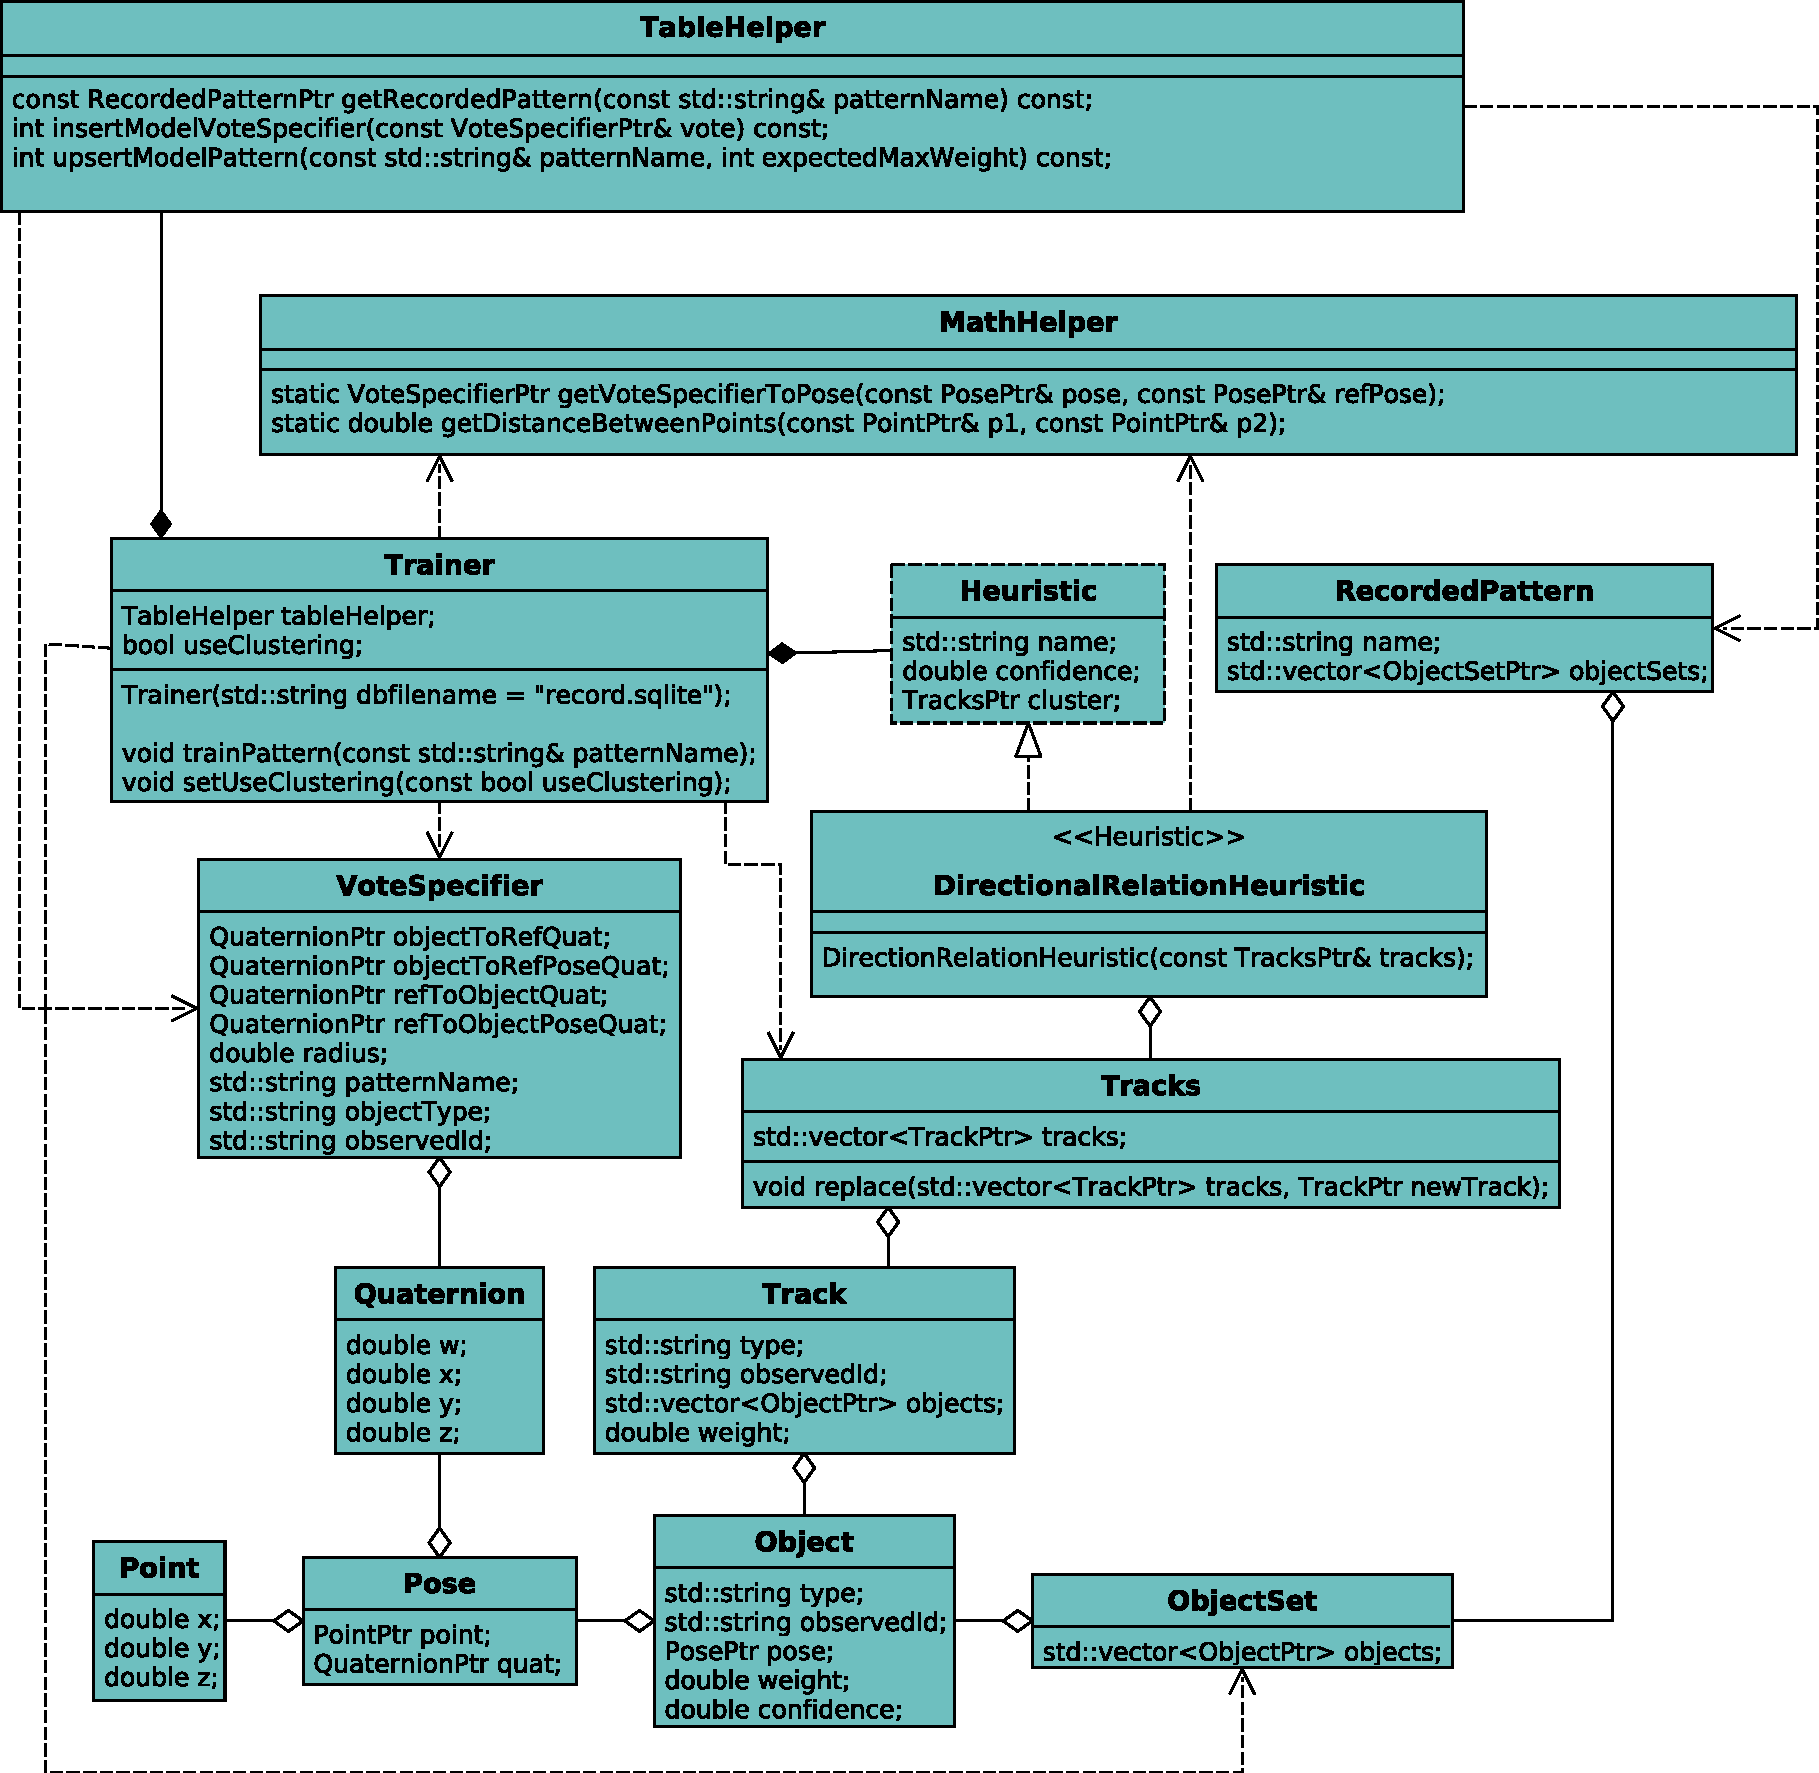
\includegraphics[width=1.0\textwidth]{uml/trainer.pdf}
  \caption{Verwendete Attribute und Funktionen im Trainingsprozess}
  \label{fig:training}
\end{figure}

Die im Trainingsprozess involvierten Klassen sind in Diagramm \vref{fig:training} ersichtlich.
Zu beachten ist, dass in der Abbildung aus Platzgründen nicht alle Klassenmethoden aufgelistet sind, sondern nur die für das Training relevanten öffentlichen Methoden und Attribute.

Die Klasse \textbf{Trainer} bildet die öffentliche Schnittstelle für den gesamten Trainingsprozess.
Die Methode \textbf{setUseClustering()} aktiviert/deaktiviert die Bildung von Hierarchien während des Trainings, sollte es mit \textbf{true} aufgerufen werden, so wird im Verlauf des Trainings die in Abschnitt \vref{ch:heuristik} beschriebenen Heuristik zur Hierarchiebildung verwendet.
Da das System auf der Grundidee beruht, dass weitere Heuristiken nach Bedarf leicht erstellt und integriert werden können, wird die abstrakte Klasse \textbf{Heuristic} als Schnittstelle für allgemeine Heuristiken eingeführt.
Die Methode \textbf{trainPattern} der \textbf{Trainer} Klasse startet den eigentlichen Trainingsvorgang für die Szene mit dem angegebenen Namen.
Sie benutzt zunächst den \textbf{TableHelper}, um mit Hilfe der Methode \textbf{getRecordedPattern()} alle Aufnahmen der genannten Szene aus der Datenbank zu laden.
Dann wird eine Spurenmenge aus den geladenen \textbf{ObjectSets} generiert, welche mit der Heuristik bewertet wird.
Dem Algorithmus \vref{algo:training} folgend, wird als Nächstes das eigentliche ISM generiert.
Für die Wahl der Referenzpose ist es notwendig, die Abstände zwischen den einzelnen Objekten einer Spur zu errechnen, wofür auf die Methode \textbf{getDistanceBetweenPoints()} der \textbf{MathHelper}-Klasse zurückgegriffen wird.

Diese stellt ebenfalls die später benötigte Funktion \textbf{getVoteSpecifierToPose()} bereit, welche die in Abschnitt \vref{ch:vote} dargestellten Berechnungen für die Erzeugung eines Votes durchführt.
Das erstellte Vote wird dann mit Hilfe der Funktion \textbf{insertModelVoteSpecifier()} in der Datenbank abgelegt.
Am Ende der Trainingsvorgangs wird mit Hilfe der Methode \textbf{upsertModelPattern()} das erwartete Gesamtgewicht der trainierten Szenen angepasst, um mit den gelernten Daten übereinzustimmen.

\subsubsection{Datenbankschema}

Ähnlich dem Recorder ist das Datenbankschema für das trainierte Modell vollständig normalisiert.
Es enthält die Tabellen \textbf{model\_votes}, \textbf{model\_objects} und \textbf{model\_patterns}.
Die Spalten der Datenbanktabellen korrespondieren dabei direkt mit den in Abschnitt \vref{ch:konzeption} dargestellten Abstraktionen und Verfahren.

\begin{description}
  \item[model\_votes] \hfill \\
    id INTEGER PRIMARY KEY, objectId INTEGER,\\ patternId INTEGER, observedId TEXT, radius FLOAT,\\ qw FLOAT, qx FLOAT, qy FLOAT, qz FLOAT,\\ qw2 FLOAT, qx2 FLOAT, qy2 FLOAT, qz2 FLOAT,\\ qpw FLOAT, qpx FLOAT, qpy FLOAT, qpz FLOAT,\\ qpw2 FLOAT, qpx2 FLOAT, qpy2 FLOAT, qpz2 FLOAT
  \item[model\_objects] \hfill \\
    id INTEGER PRIMARY KEY, type TEXT UNIQUE
  \item[model\_patterns] \hfill \\
    id INTEGER PRIMARY KEY, name TEXT UNIQUE,\\ expectedMaxWeight INTEGER
\end{description}

Für zu speichernde Votes wird erst sichergestellt, dass die entsprechende Szenendefinition in der \textbf{model\_patterns} Tabelle und die entsprechende Objektdefinition in der \textbf{model\_objects} Tabelle vorhanden sind.
Dann wird die zum im Vote vermerkten Szenennamen passende \textbf{patternId} beziehungsweise zum votenden Objekttyp gehörende \textbf{objectId} zusammen mit den serialisierten Votedaten in der \textbf{model\_votes} Tabelle abgelegt.
Wie in Abschnitt \vref{ch:impl-training} beschrieben wird am Ende des Trainingsprozesses mit der \textbf{upsertModelPattern()} Funktion der \textbf{TableHelper} Klasse der Wert \textbf{expectedMaxWeight} der gespeicherten Szene aktualisiert.

\subsection{Recognizer}

\begin{figure}
  \centering
  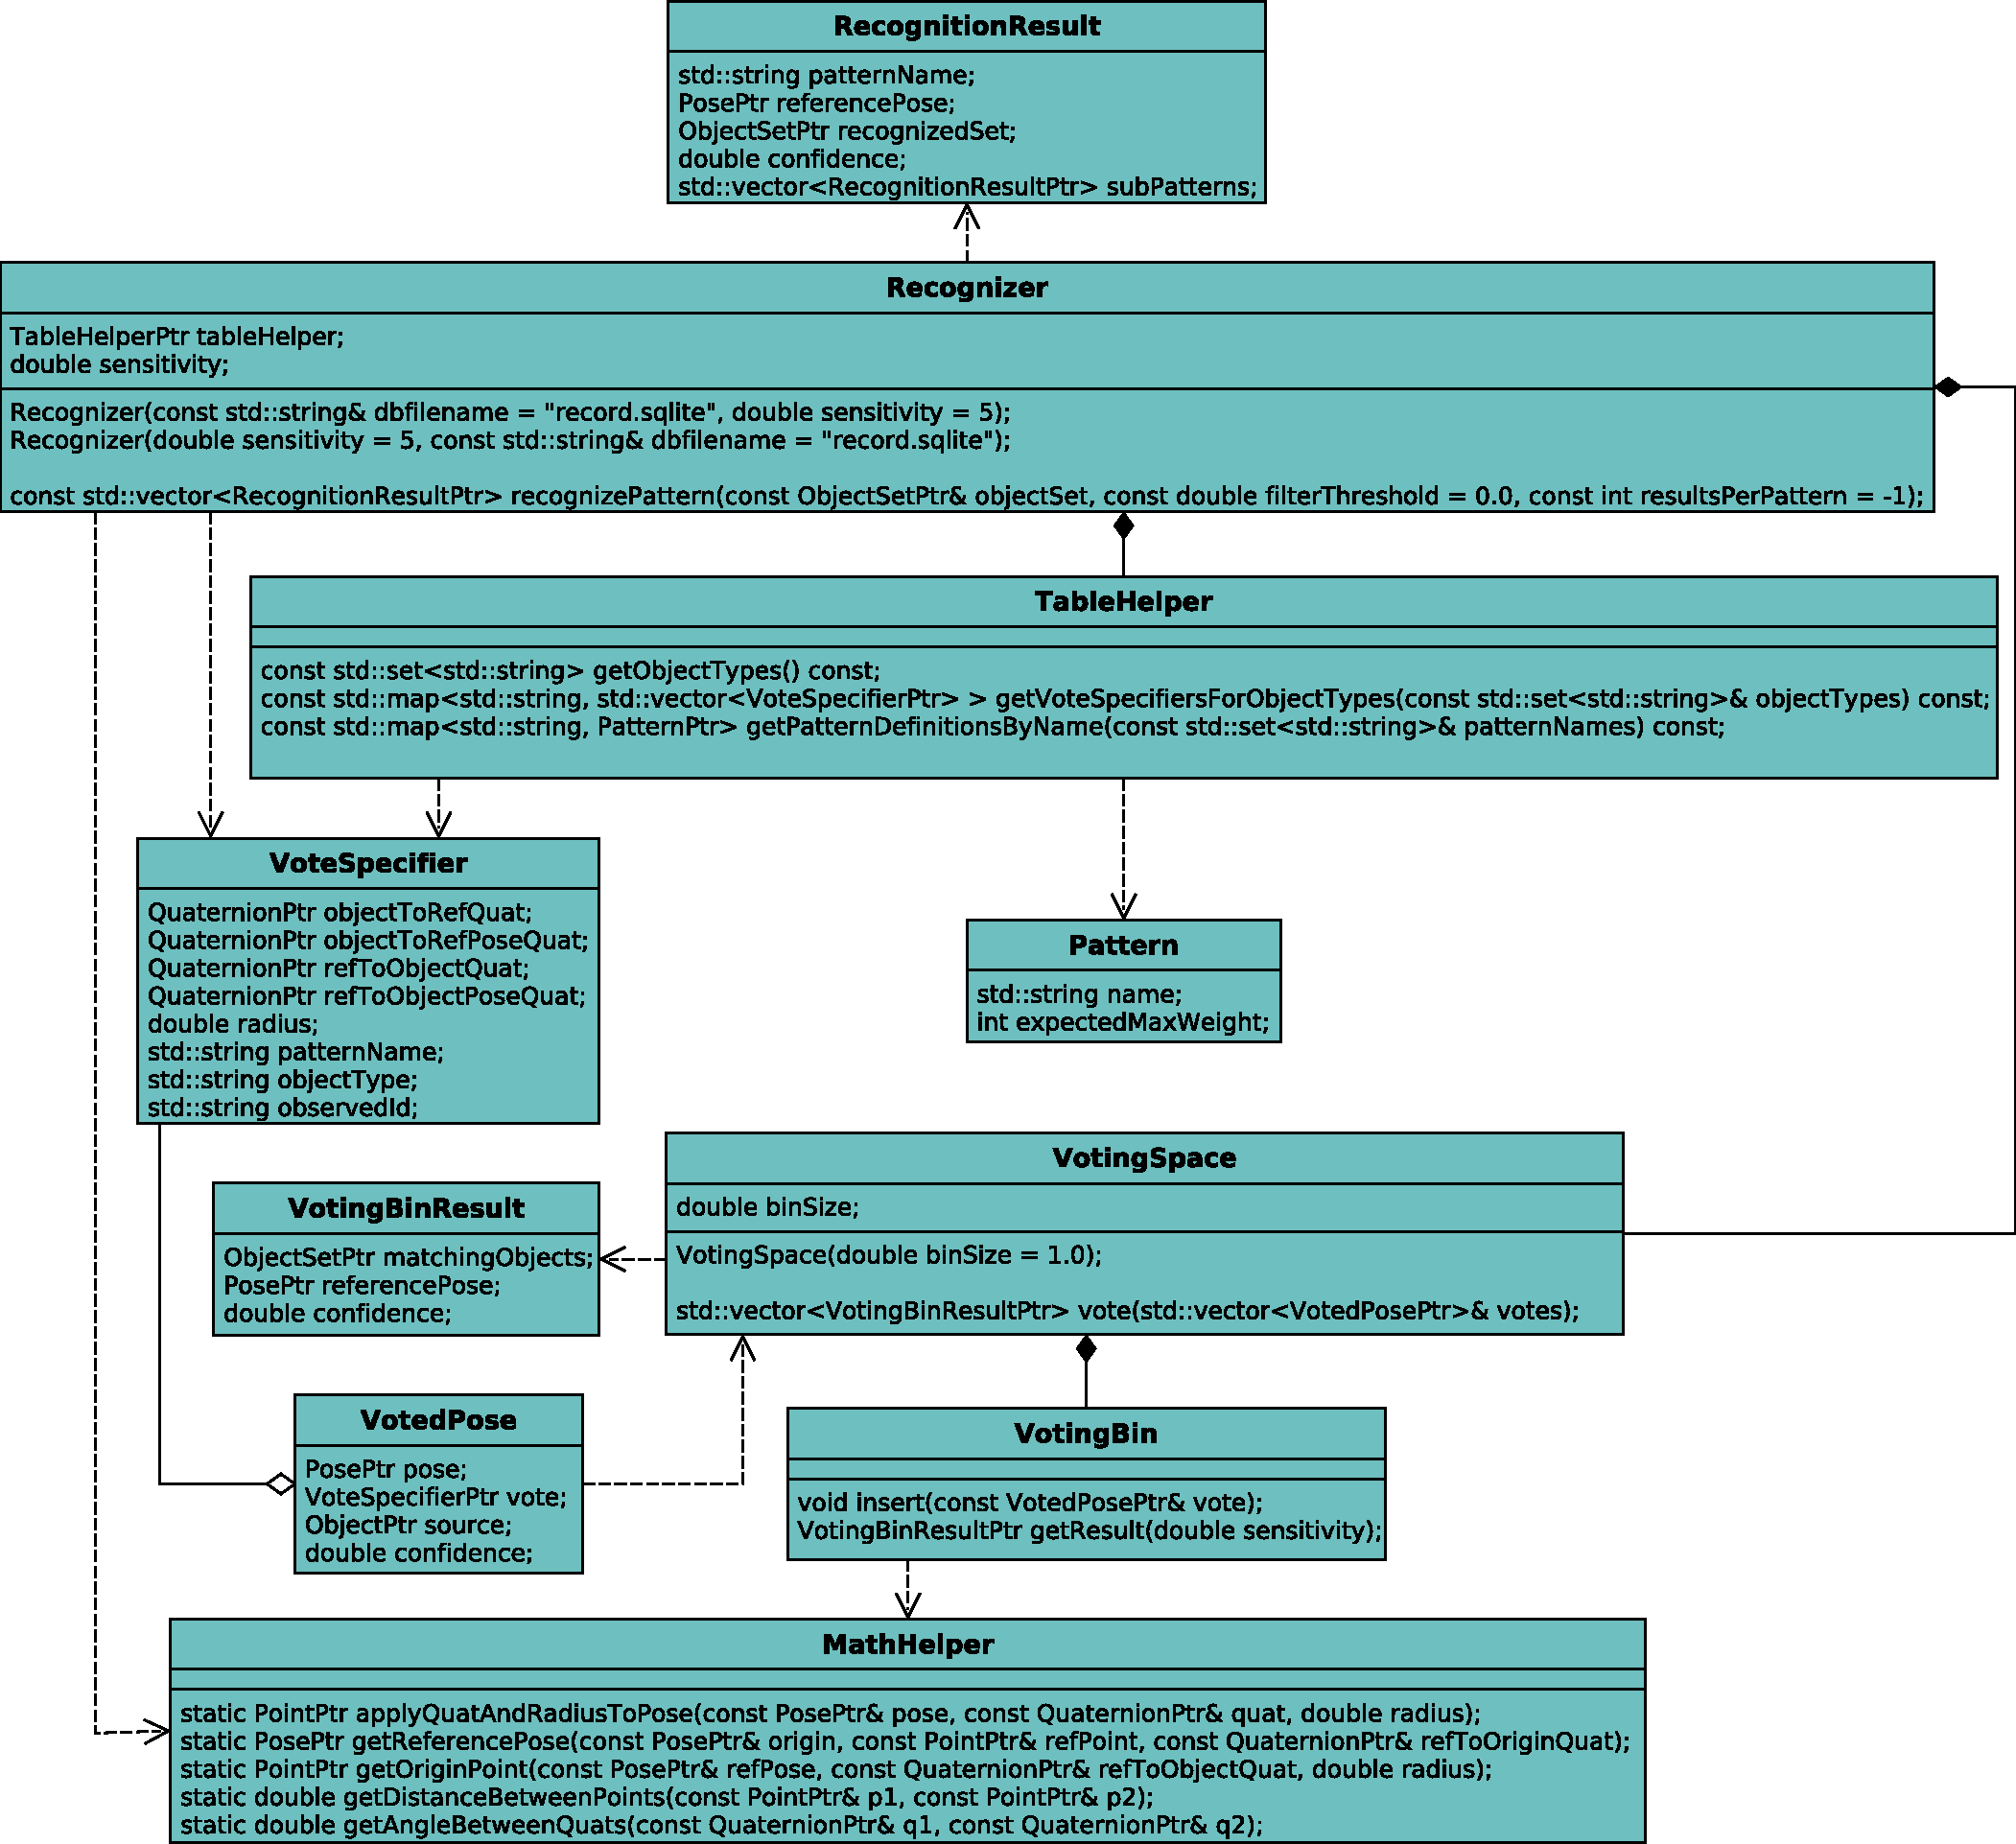
\includegraphics[width=1.0\textwidth]{uml/recognizer.pdf}
  \caption{Verwendete Attribute und Funktionen im Erkennungsprozess}
  \label{fig:recognizer}
\end{figure}

Die \textbf{Recognizer} Klasse bildet die öffentliche Schnittstelle des eigentlichen Erkennungsverfahrens.
Es besitzt neben dem Konstruktor nur eine weitere Methode namens \textbf{recognizePattern()}, welche als Eingabe ein \textbf{ObjectSet} erhält.
Dieses \textbf{ObjectSet} enthält erkannte Objekte aus einem beliebigen vorgeschalteten Erkennungsverfahren.
Der Rückgabewert der \textbf{recognizePattern()}-Methode besteht aus einem \textbf{vector} von \textbf{RecognitionResult} Containern.
Diese enthalten den Namen der erkannten Szene, ihre Referenzpose, ein \textbf{ObjectSet} mit den in der Eingabemenge erkannten Objekten, sowie eine Konfidenz und die Menge \textbf{subPatterns}.
Die \textbf{subPatterns}-Menge ist nur dann nicht leer, wenn im Trainingsprozess erfolgreich Heuristiken angewandt wurden.
Sie enthält für jeden durch einen Heuristik erkannten Zusammenhang das Sub-ISM, welches aus den durch die Heuristik gewählten Unterobjekten besteht.

Dem Algorithmus \vref{algo:erkennung-main} folgend, werden zuerst mit Hilfe der Funktionen \textbf{getVoteSpecifiersForObjectTypes()} der \textbf{TableHelper}-Klasse die Votes der an der Eingabemenge beteiligten Objekttypen geladen.
Sollte ein Objekt der Eingabemenge keinen erkannten Objekttyp aufweisen, so werden mit der Funktion \textbf{getObjectTypes()} zunächst alle vorhandenen Objekttypen geladen, um in Kombination mit der vorangegangenen Funktion sämtliche Votes aus der Datenbank extrahieren zu können.
Da in den folgenden Schritten für jede Szene separat gevoted wird, ist es nötig für jeden zu votenden Szenennamen mittels der Funktion \textbf{getPatternDefinitionsByName()} die entsprechenden Szenendefinitionen zu laden.
Diese werden benötigt um für die errechneten angewandten Votes die passenden Gewichte zu verteilen.
Um die eigentlichen angewandten Votes zu berechnen, bedient sich der \textbf{Recognizer} der Funktionen \textbf{applyQuatAndRadiusToPose()} sowie \textbf{getReferencePose()} der \textbf{MathHelper}-Klasse.

Zur Einleitung der Aggregations- und Rückprojektionsphase werden die angewandten Votes für jeden Szenentyp einzeln der Klasse \textbf{VotingSpace} übergeben.
Dies geschieht durch Aufruf der Funktion \textbf{vote}, welcher ein \textbf{vector} angewandter Votes übergeben wird.
Der \textbf{VotingSpace} führt die eigentliche Diskretisierung des Raumes in Buckets durch.
Jeder Bucket ist durch eine Instanz der Klasse \textbf{VotingBin} repräsentiert, auf der für jedes Vote die \textbf{insert()} Methode aufgerufen wird.
Nachdem alle Votes in die \textbf{VotingBins} eingefügt wurden, wird für jeden Bucket die Funktion \textbf{getResults()} aufgerufen, welche die Einpassung anstößt und das Einpassungsergebnis zurückliefert.
Um die für die Einpassung notwendigen Berechnungen durchzuführen bedient sich die Klasse der Hilfsfunktionen \textbf{getOriginPoint()}, \textbf{getDistanceBetweenPoints()} sowie \textbf{getAngleBetweenQuats()} der \textbf{MathHelper}-Klasse.

\section{Hilfsprogramme für das Terminal}

Um das Arbeiten mit den entwickelten Komponenten zu erleichtern, wurden einige Hilfsprogramme für das Linux-Terminal entwickelt.

\paragraph{trainer}

Das wichtigste Hilfsprogramm ist der \textbf{trainer}.
Es wird benutzt um den Trainingsprozess für die aufgenommenen Daten anzustoßen.

\paragraph{dataMerger}

Der \textbf{dataMerger} kann genutzt werden um Aufnahmen und trainierte Modelle zwischen Datenbanken zu übertragen und um mehrere Datenbanken in einer zu vereinen.

\paragraph{modelCleaner}

Der \textbf{modelCleaner} wird benutzt um alle bestehenden Modelle aus der Datenbank zu löschen.
Dies ist immer dann notwendig, wenn ein bereits trainiertes Modell mit neuen Daten aus der Aufnahme ergänzt werden soll, sich die alten Aufnahmedaten aber noch in der Datenbank befinden.
Würde dann nochmals trainiert, würden die alten Aufnahmedaten der Datenbank doppelt hinzugefügt. Dies würde die Geschwindigkeit der Erkennung durch die höhere Anzahl an gespeicherten Votes potentiell drastisch verringern.

\paragraph{validator}

Dieses Hilfsprogramm wird primär zum Debugging verwendet.
Es greift auf eine Datenbank mit sowohl Aufnahme- als auch Modelldaten einer Szene zu und versucht die Aufnahmedaten anhand des generieren Modells wiederzuerkennen.
Dabei kann es optional den Typ sowie den Identifikator der Objekte in den Aufnahmedaten vor der Erkennung löschen, um eine Erkennung mit weniger Informationsgehalt zu testen.
Über das Programm können auch nur Ausschnitte der Aufnahmedaten für die Wiedererkennung genutzt und auch die Bucketgröße konfiguriert werden.
Am Ende des Validierungsdurchlaufs gibt das Programm einen Durchschnittswert der Erkennungskonfidenzen aus.
Sollte eine Erkennung mit gelöschtem Typ/ID gewählt worden sein, wird zusätzlich noch eine Zusammenfassung über die Identifizierungsrate der beteiligten Objekte ausgegeben.

\paragraph{testRunner}\label{impl:testrunner}

Der \textbf{testRunner} wird benutzt, um die Leistung des Verfahrens unter verschiedenen Umständen zu messen.
Er generiert verschiedene Erkennungsszenarien aus einer größeren Aufnahme und misst die Laufzeit der Erkennung unter Veränderung von Typ/ID-Informationen, Bucketgröße, Anzahl an trainierten Sets, Anzahl an trainierten Objekten sowie aktiviertem und deaktiviertem hierarchischem Clustering.
Die Messwerte werden dann für eine spätere Auswertung in einer CSV-Datei gespeichert.
Das Format der CSV-Datei ist durch die erste Zeile gegeben und lautet:\\
\emph{setCount, objectCount, sensitivity, useClustering, useType, useId, runtime, confidence}

\section{Visualisierung}\label{impl:visualisierung}

\begin{figure}
  \centering
  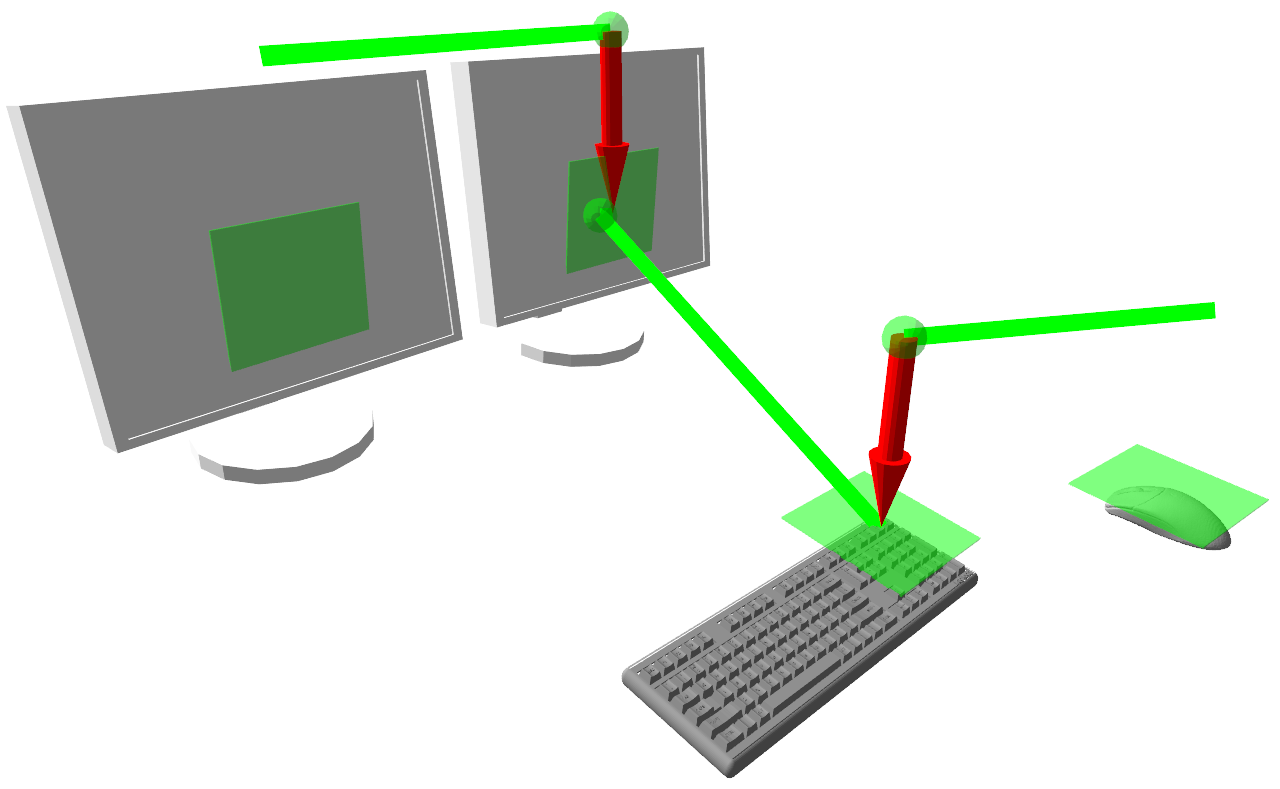
\includegraphics[width=0.7\textwidth]{bilder/paper_fotos/s1.png}
  \caption{Visualisierung einer Szenenerkennung. Bildquelle: \cite{P.MeissnerandR.RecklingandR.JaekelandS.R.Schmidt-RohrandR.Dillmann2013}}
  \label{fig:visualisierung}
\end{figure}

Aufbauend auf dem RViz-Paket des Robot Operating Systems und den bisher beschriebenen Programmkomponenten wurde eine dreidimensionale Visualisierung der Erkennungsergebnisse entwickelt.
Diese läuft als eigenständiger ROS-Knoten und zeichnet parallel zu bestehenden Objektvisualisierungen das Erkennungsergebnis an die passenden Positionen.
Im Falle von erkannten Clustern werden die Beziehungen einzelner Teilszenen zueinander hervorgehoben.
Ein Beispiel für die Visualisierung ist in Abbildung \vref{fig:visualisierung} ersichtlich.
Dabei ist zu beachten dass für die dargestellte Visualisierung Marker für die Objekterkennung verwendet wurden, welche in der Visualisierung um Modelle der echten Objekte wie Maus/Tastatur ergänzt wurden.

Visualisiert wird jeweils das beste Erkennungsergebnis.
Die Qualität des Ergebnisses ist durch die Farbe der Verbindungslinien gegeben.
Ein helles Grün steht für eine sehr sichere Erkennung. Je weiter der Farbton in den roten Bereich wechselt, desto niedriger ist die Erkennungskonfidenz.
Die großen roten Pfeile in der Visualisierung repräsentieren die Referenzpunkte von Subszenen.
In dem gegebenen Beispiel ist zu erkennen, dass sowohl die beiden Monitore, als auch Maus und Tastatur jeweils ein durch die direktionale Heuristik gegebenes Sub-ISM bilden.
Die beiden Unterszenen sind dann wiederum durch den rechten Monitor sowie die Tastatur miteinander verbunden.
Daraus ist zu erkennen, dass der rechte Monitor als Referenzobjekt der linken und die Tastatur als Referenzobjekt der rechten Subszene gewählt wurde.
